
\typeout{}\typeout{If latex fails to find aiaa-tc, read the README file!}
%


\documentclass[]{aiaa-tc}% insert '[draft]' option to show overfull boxes

\usepackage{mathptmx}         %CHANGE FONT TO TIMES NEW ROMAN

\usepackage{amsmath}          % for formula writing (i.e. 'split', etc)
\usepackage{rotate}           %rotate/mirror images
\usepackage{cancel}           %draw lines through math to show "goes to zero"
\usepackage{xfrac}            %allows slated and side fractions
\usepackage{subcaption}       %allows captioning individual subfigures
\usepackage{multicol}         %enable environment with multiple columns
\usepackage[mode=buildnew]{standalone}% requires -shell-escape
  % compile with `pdflatex -shell-escape main` or `xelatex  -shell-escape main`


\usepackage{tikz}             %for creating vector graphics diagrams
\usetikzlibrary{backgrounds}  %put backgrounds behind tikz figures
\usetikzlibrary{calc}         %perform calculations within $$
\usetikzlibrary{positioning}  %position tikz elements using "right of, etc"
\usetikzlibrary{angles}       %label angles between lines with arcs
\usetikzlibrary{quotes}       %Put angle label in quotes
\usetikzlibrary{patterns}     %Patterns to fill shapes with




  \title{MAE 298 Aeroacoustics -- Homework\#4 \\ Turbomachinery Noise}


\author{
  Logan D. Halstrom \\
  {\normalsize\itshape Graduate Student} \\
  {\normalsize\itshape Department of Mechanical and Aerospace Engineering} \\
  {\normalsize\itshape University of California, Davis, CA 95616}
       }


 % Define commands to assure consistent treatment throughout document
 \newcommand{\eqnref}[1]{(\ref{#1})}
 \newcommand{\class}[1]{\texttt{#1}}
 \newcommand{\package}[1]{\texttt{#1}}
 \newcommand{\file}[1]{\texttt{#1}}
 \newcommand{\BibTeX}{\textsc{Bib}\TeX}



%%%%%%%%%%%%%%%%%%%%%%%%%%%%%%%%%%%%%%%%%%%%%%%%%%%%%%%%%%%%%%%%%%%%%%%%
\begin{document}

\maketitle


% % %%%%%%%%%%%%%%%%%%%%%%%%%%%%%%%%%%%%%%%%%%%%%%%%%%%%%%%%%%%%%%%%%%%%%%%%
% \begin{abstract}

% Abstract about lit study

% \end{abstract}





% %%%%%%%%%%%%%%%%%%%%%%%%%%%%%%%%%%%%%%%%%%%%%%%%%%%%%%%%%%%%%%%%%%%%%%%%
% \section*{Nomenclature}

% \begin{multicols}{2}

% \begin{tabbing}
%   XXX \= \kill% this line sets tab stop
%   $0$                 \> Subscript for quiescent parameters \\
%   $e$                 \> Subscript for emission parameters \\
%   $L$                 \> Subscript for loading parameters \\
%   $t$                 \> Time \\
%   $\tau$              \> Retarded time \\
%   $ret$               \> Evaluated at retarded time \\
%   $\hat{n}$           \> Unit surface normal vector \\
%   $\vec{r}$           \> Radial direction vector \\
%   $\hat{r}$           \> Radial unit vector \\
%   $r$                 \> Magnitude of radial vector $|\vec{r}|$ \\
%   $\theta$            \> Angle between $\hat{n}$ and $\hat{r}$ \\
%   $f$                 \> Function of surfaces within a fluid space \\
%   $\vec{V}$           \> General velocity vector \\
%   $V_r$               \> Velocity component in radial direction \\
%   $V_n$               \> Velocity component in surface normal direction \\
%   $M$                 \> Mach number \\
%   $c$                 \> Speed of Sound\\
%   $\overline{\rho}$   \> Mean density \\
%   $p$                 \> Pressure  \\
%   $\widetilde{p}$     \> Pressure (Discontinuous across data surface)  \\
%   $\overline{p}$      \> Mean pressure \\
%   $p'$                \> Perturbation pressure \\
%   $\Delta P$          \> Pressure difference from CFD solution \\
%   $L$                 \> Pressure loading \\
%   $\overline{\partial}$ \> Generalized derivative \\
%   $\delta$            \> Dirac delta function \\
%   \scriptsize{FW-H}   \> Ffowcs Williams-Hawkings\\






% \end{tabbing}

% \end{multicols}


%%%%%%%%%%%%%%%%%%%%%%%%%%%%%%%%%%%%%%%%%%%%%%%%%%%%%%%%%%%%%%%%%%%%%%%%
\section*{Problem Statement}
%%%%%%%%%%%%%%%%%%%%%%%%%%%%%%%%%%%%%%%%%%%%%%%%%%%%%%%%%%%%%%%%%%%%%%%%

You are designing a new aircraft engine and analyzing acoustic propagation generated by a non-uniform flow with angle of attack interacting with rotating fans. You obtained flow fields from CFD for a one-sixth small scale of the engine. The radius for the small scale engine is 13 in and the hub radius is 3 in. CFD provides the velocity gust information as a function of its circumferential modes. The circumferential mode for acoustics can be expressed as $m = nB − kV$ where $B$ is the number of blades, $V$ is the number of vanes, $n$ stands for the harmonic of BPF and $k$ is the integer (1, 2, 3...). You consider only positive $k$ at this time (this is related the rotation direction of gust). The number of blades is 18. The number of vanes is considered to be 1 since there is no physical vanes but there is one revolution difference. The Mach number is 0.525 and the fan RPM is 8326.3042, the speed of sound is 13503.937009 in/s and the density is 1.4988E-5 slug/in\^3. The dominant noise is generated at the 1st BPF or $n=1$ in which the
angular frequency $\omega$ is given as $RPM \times \frac{2\pi}{60}\times B$. We are interested in the propagation through the inlet of !"
the engine so that sound propagates to $–z$ direction assuming the $+z$ direction is in the flow direction.



%%%%%%%%%%%%%%%%%%%%%%%%%%%%%%%%%%%%%%%%%%%%%%%%%%%%%%%%%%%%%%%%%%%%%%%%
\section{Eigenvalues}
%%%%%%%%%%%%%%%%%%%%%%%%%%%%%%%%%%%%%%%%%%%%%%%%%%%%%%%%%%%%%%%%%%%%%%%%

1. [20 points] Determine the first five eigenvalues of acoustics for m=18, 17, 16, 15 or (k=1, 2, 3, 4) or (m,n)=(18,0), (18,1), (18,2), (18,3), (18,4), (17,0), (17,1), (17,2), (17,3), (17,4), (16,0), (16,1), (16,2), (16,3), (16,4), (15,0), (15,1), (15,2), (15,3), (15,4)

\begin{center}
\begin{table}[htb]
\begin{tabular}{| c | c c c c |}
\hline
% {} & \multicolumn{4}{c}{m} \\
{} &  $\mathbf{m=18}$ &  $\mathbf{m=17}$ &  $\mathbf{m=16}$ &  $\mathbf{m=15}$ \\
\hline
$\mathbf{n=0}$ &       1.549545 &       1.469574 &       1.389482 &       1.309256 \\
$\mathbf{n=1}$ &       1.961197 &       1.875532 &       1.789559 &       1.703250 \\
$\mathbf{n=2}$ &       2.282319 &       2.193182 &       2.103645 &       2.013674 \\
$\mathbf{n=3}$ &       2.577225 &       2.485453 &       2.393227 &       2.300507 \\
$\mathbf{n=4}$ &       2.858492 &       2.764587 &       2.670191 &       2.575265 \\
\hline
\end{tabular}
\caption{test}
\end{table}
\end{center}





%%%%%%%%%%%%%%%%%%%%%%%%%%%%%%%%%%%%%%%%%%%%%%%%%%%%%%%%%%%%%%%%%%%%%%%%
\subsection{Ground Testing}

The most straight-forward of testing methods described by Himelblau is the




% %%\vspace{-2em}
% \begin{figure}[tb!]
% \begin{center}
% 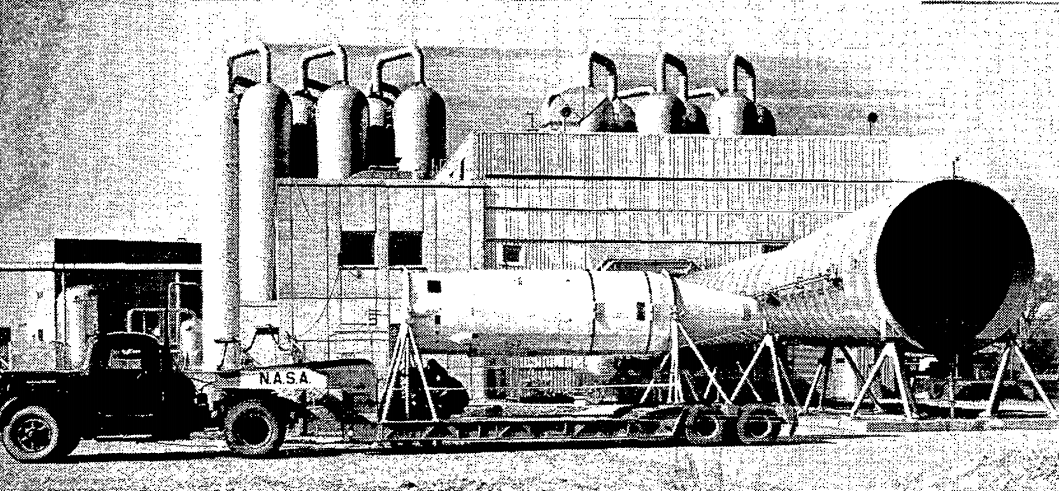
\includegraphics[width=\textwidth]{Images/Himelblau_Fig36.png}
% \caption{Acoustic test of the OGO spacecraft near the discharge nozzle of a large blowdown wind tunnel\cite{SpaceVehicleAeroacousticVibrationPrediction}}
% \label{FreeFieldTest}
% \end{center}
% \end{figure}
% %%\vspace{-2em}






%%%%%%%%%%%%%%%%%%%%%%%%%%%%%%%%%%%%%%%%%%%%%%%%%%%%%%%%%%%%%%%%%%%%%%%%
\section{Eigenfunctions}
%%%%%%%%%%%%%%%%%%%%%%%%%%%%%%%%%%%%%%%%%%%%%%%%%%%%%%%%%%%%%%%%%%%%%%%%

2. [20 points] Plot the five eigenfunctions (radial modes, n=0, 1, 2, 3, 4) for m=18, 17, 16, 15 or (k=1, 2, 3, 4) and verify n describes the number of zero crossings in the radial direction

%%%%%%%%%%%%%%%%%%%%%%%%%%%%%%%%%%%%%%%%%%%%%%%%%%%%%%%%%%%%%%%%%%%%%%%%
\section{Wavenumbers}
%%%%%%%%%%%%%%%%%%%%%%%%%%%%%%%%%%%%%%%%%%%%%%%%%%%%%%%%%%%%%%%%%%%%%%%%

3. [20 points] Determine the wavenumbers in the z direction for (m,n)=(18,0), (18,1), (18,2), (17,0), (17,1), (17,2), (16,0), (16,1), (16,2), (15,0), (15,1), (15,2). Indicate whether the mode is cut-on (propagating) or cut-off (exponentially decaying). Consider only the propagation in the –z direction. Exclude the exponentially growing solution and include only the propagating solutions or exponentially decaying solutions.


\begin{tabular}{| c c c c |}
\hline
$\mathbf{m}$ &  $\mathbf{n}$ &                      $\mathbf{Kz}$ & $\mathbf{Cut-on}$ \\
\hline
18 &             0 &  (-0.842342752252+0.860467931211j) &                No \\
18 &             1 &    (-0.842342752252+1.6539375966j) &                No \\
18 &             2 &   (-0.842342752252+2.14865069168j) &                No \\
\hline
17 &             0 &  (-0.842342752252+0.63804009925j) &                No \\
17 &             1 &   (-0.842342752252+1.5105548176j) &                No \\
17 &             2 &  (-0.842342752252+2.01642513534j) &                No \\
\hline
16 &             0 &  (-0.842342752252+0.301624659942j) &                No \\
16 &             1 &   (-0.842342752252+1.35896420335j) &                No \\
16 &             2 &    (-0.842342752252+1.8801224576j) &                No \\
\hline
15 &             0 &              (-0.386366560427+0j) &               Yes \\
15 &             1 &  (-0.842342752252+1.19608312922j) &                No \\
15 &             2 &  (-0.842342752252+1.73881279925j) &                No \\
\hline
\end{tabular}






%%%%%%%%%%%%%%%%%%%%%%%%%%%%%%%%%%%%%%%%%%%%%%%%%%%%%%%%%%%%%%%%%%%%%%%%
\section{Modal Power Levels}
%%%%%%%%%%%%%%%%%%%%%%%%%%%%%%%%%%%%%%%%%%%%%%%%%%%%%%%%%%%%%%%%%%%%%%%%

4. [30 points] The pressure distribution file at z=0 plane for m=18 or 1 BPF is provided. The first column is the dimensional radius [in], the second column the real part of the pressure [psi], and the third column is the imaginary part of the pressure [psi]. Using this boundary condition, compute the sound power level for (m,n)=(18,0), (18,1), (18,2). This noise is considered for blade self noise that is not associated with the gust response since k=0. Note that the z=0 plane is not the same as the engine inlet. Use the conversion for the unit for the sound power as follows: PWL (dB)=10*log10((Wmn))- 10*log10(7.3756E-13)
















\end{document}


